% Ready-to-paste figure blocks for Results.tex (not \input anywhere yet).
% Figures are made by Report/figures/results/make_results_plots.py from logs
% already in BenchTest/logs; every number below was printed by that script.

% ---------------------------------------------------------------------------
% 1. IMU interval at flash writes (v0.5.0 vs v0.6.0)
% ---------------------------------------------------------------------------
Figure~\ref{fig:res-imu-gaps} shows the longest sample interval in each 2\,s window. With v0.5.0 (29 September), 30 of the 151 logging-on windows per IMU had a maximum interval of 33.0 to 40.0\,ms, one about every 10\,s, and in the 59 windows with flash logging off the worst interval was 5.9\,ms. With buffered writes in v0.6.0 (1 October) only 5 of 173 windows per IMU exceeded 10\,ms (37.3 to 40.1\,ms), each in the first window reported after one of the five flushes, and the worst interval elsewhere was 5.9\,ms; no sample was dropped in either run.

\begin{figure}[htbp]
\centering
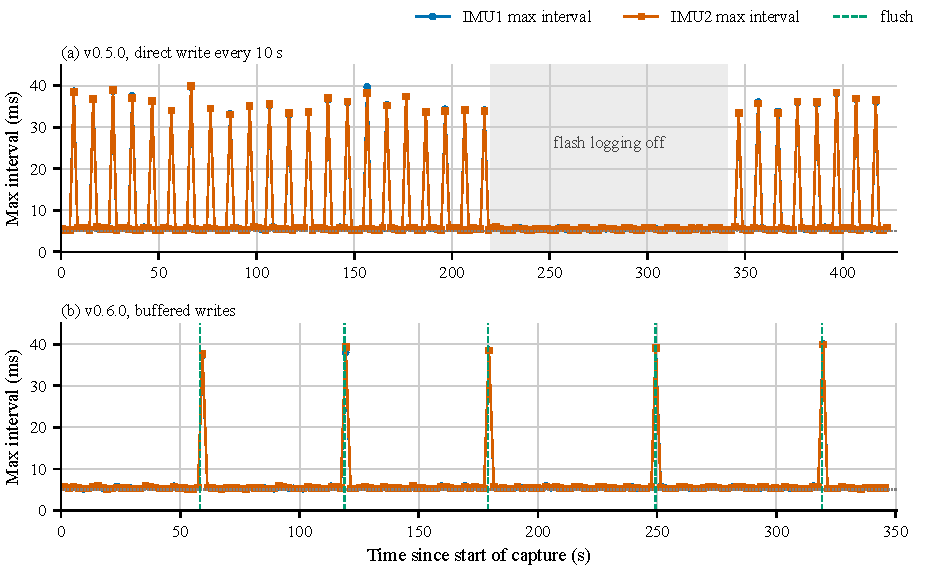
\includegraphics[width=\textwidth]{figures/results/imu_write_gaps.pdf}
\caption{Longest interval between consecutive IMU samples in each 2\,s statistics window, on the bench. (a) Firmware v0.5.0, 29 September, writing to flash every 10\,s; the grey band is the period with flash logging switched off (219.7 to 340.8\,s). (b) Firmware v0.6.0, 1 October, buffered logging; dashed lines mark the five flushes as logged by the firmware (71 to 202\,ms each). The firmware reports only the minimum, mean and maximum interval per window, so each point is one window maximum (212 windows per IMU in (a), 173 in (b)); times are when the host received the line. The dotted line is the nominal 5\,ms interval at 200\,Hz. No samples were dropped in either run.}
\label{fig:res-imu-gaps}
\end{figure}

% ---------------------------------------------------------------------------
% 2. Detector latency, Pi 4 and Pi 5
% ---------------------------------------------------------------------------
Figure~\ref{fig:res-latency} compares the per-frame time from sensor readout to detection result. On the Pi~4 with four inference threads the median was 102\,ms (95th percentile 120\,ms, 1161 frames) and 105\,ms with the live view open (127\,ms, 1031 frames); with one thread it rose to 186\,ms (207\,ms, 419 frames) as inference went from 36 to 126\,ms. The Pi~5 on 15 October had a median of 53\,ms and a 95th percentile of 62\,ms over 1151 frames, with inference at 28\,ms and queue wait at 18\,ms against 52\,ms on the Pi~4. The 11 October whole-system log on the Pi~4 (bridge, fusion and preview running) recorded only per-interval summaries, median 118 to 122\,ms and 95th percentile 146 to 148\,ms, so it is not plotted.

\begin{figure}[htbp]
\centering
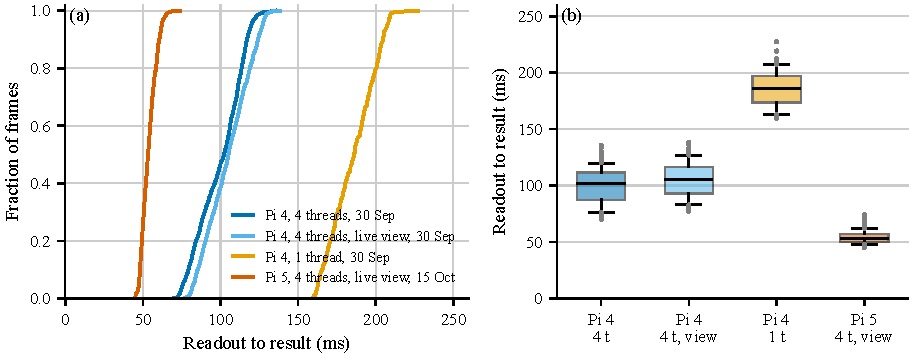
\includegraphics[width=\textwidth]{figures/results/detector_latency.pdf}
\caption{Detector latency from camera readout to detection result, per frame, for 60\,s runs of the TensorFlow Lite detector (\texttt{detect.tflite}, 300$\times$300 input, 640$\times$480 camera stream). (a) Cumulative distribution; (b) box plots with the box at the quartiles, whiskers at the 5th and 95th percentiles and dots beyond them. Pi~4 runs on 30 September: four threads (1161 frames, 19.5 frames/s), four threads with the live view open in the Pi's browser (1031 frames, 17.3 frames/s), one thread (419 frames, 7.0 frames/s). Pi~5 run on 15 October: four threads with the live-view server running (1151 frames, 19.3 frames/s). Data from the detector's per-frame timing CSV files.}
\label{fig:res-latency}
\end{figure}

% ---------------------------------------------------------------------------
% 3. Road session, 19 October
% ---------------------------------------------------------------------------
Figure~\ref{fig:res-road} shows the 19 October session from the rear unit's telemetry. After removing repeats there were 3464 records between sequence numbers 4549 and 10105, so 2093 of 5557 (37.7\,\%) were not received: 407 in one gap from 18:06:34 to 18:13:23, the rest in short gaps of at most 8 records. Vibration stayed near 0.03\,m/s$^2$ (median 0.030) while parked and had a median of 1.39\,m/s$^2$ (maximum 5.09) in the 607 records flagged as driving, and the battery current reached $-46.9$\,A with a median of $-6.3$\,A over the 307 records above 1\,A.

\begin{figure}[htbp]
\centering
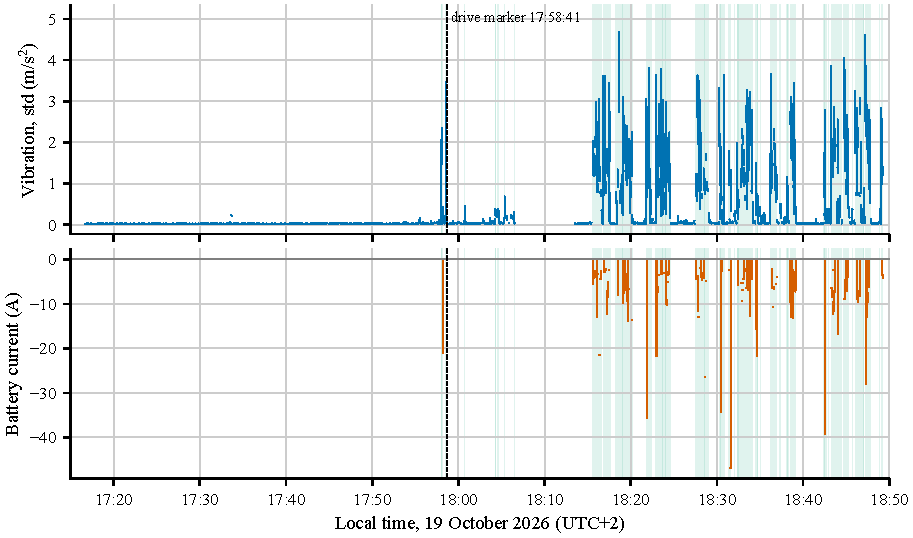
\includegraphics[width=\textwidth]{figures/results/road_session_1019.pdf}
\caption{Road session on 19 October 2026, 17:15 to 18:50 local time (UTC+2), from the rear Raspberry Pi's recorder file \texttt{2026-10-19\_171534\_roadtest.jsonl}. Top: vibration value (standard deviation of the fused acceleration magnitude per 1\,s window). Bottom: battery current from the BMS, negative for discharge. The recorder polled twice a second and the bridge repeats the latest record, so the 10\,287 rear rows carrying a telemetry record were reduced to 3464 by keeping the first row for each sequence number. Lines break wherever a sequence number is missing (2093 of 5557, 37.7\,\%, including one gap of 407 records from 18:06:34 to 18:13:23). Green shading marks records with $|i|>1$\,A or vibration above 0.3\,m/s$^2$ (607 records); the dashed line is the drive marker added from the laptop at 17:58:41.}
\label{fig:res-road}
\end{figure}

% ---------------------------------------------------------------------------
% 4. Store-and-forward outage test T15, 11 October
% ---------------------------------------------------------------------------
Figure~\ref{fig:res-t15} shows the backlog during T15. With the radio off for 600\,s the backlog grew by one record every 10\,s to 60 records, MQTT reconnected 5.2\,s after the radio was switched back on, and the backlog was cleared 37.9\,s later. On the server side the 60 replayed records arrived over 37.3\,s (1.6 records/s), and the database held all 112 records expected for the boot (sequence 65 to 176) with no duplicates and none missing.

\begin{figure}[htbp]
\centering
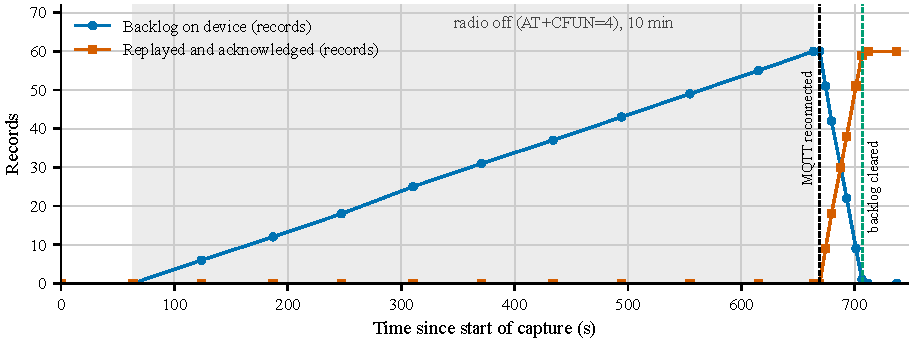
\includegraphics[width=\textwidth]{figures/results/t15_outage_backlog.pdf}
\caption{Store-and-forward outage test T15 on the bench, 11 October, firmware v0.7.4. The radio was turned off with \texttt{AT+CFUN=4} at 63.4\,s and back on with \texttt{AT+CFUN=1} at 663.7\,s (grey band); the board was not reset. Points are the device's own counters from the 21 \texttt{!sync} status lines in the capture: records stored on the device and not yet acknowledged (backlog), and records replayed and acknowledged since the outage began. Dashed lines mark the MQTT reconnection (669.0\,s) and the firmware's ``backlog cleared'' message (706.9\,s). The server's per-record receive times were not exported for this run, so the figure uses the device counters; the server-side totals are in the text.}
\label{fig:res-t15}
\end{figure}
